\chapter{Funktionen}\label{ch:K04_Functions}

\section{Eigene Funktionen  definieren}

In den vergangenen Lektionen haben Sie bereits viele Funktionen (=Befehle) verwendet, wie beispielsweise \lstinline|t.forward(100)| oder \lstinline|print()|. Im Allgemeinen erkennen Sie Befehle daran, dass Sie mit einem \textbf{Wort} beginnen, wie beispielsweise \lstinline|t.forward| oder \lstinline|print|, auf welches Klammern sowie ein oder mehrere Werte folgen. Diese Werte werden \textbf{Parameter} genannt und dienen dazu, das Verhalten einer Funktion leicht abzuändern, so dass beispielsweise in der Funktion \lstinline|t.fd()| 50 oder 100 Pixel gezeichnet werden. Um unseren Code leserlicher und kürzer zu machen, können wir auch eigene Definitionen schreiben!

\begin{myexample}
Wir betrachten nochmals den Code aus \cref{myexercise:Blume}:

\lstinputlisting[language=Python,caption=\texttt{blume.py},label=listing:blume2]{Grundlagen_Info/00_Programmieren/Skript/Code/K02_Intro/blume.py}

Wir könnten den Code leserlicher machen, indem wir einen Befehl für eine Quadrat und einen Befehl für das gesamte Muster erstellen:

\begin{minipage}{\linewidth}
	\begin{figure}[H] % not really a figure, just acts as non-floating container
		\begin{lstlisting}[escapechar=!, numbers=left]
import turtle as t

def !\colorbox{HotPink}{viereck()}!: !\tikzmark{to2ex}!
    for _ in range(4):
        t.fd(100)
        t.rt(360/4)

def !\colorbox{CornflowerBlue}{viereck\_blume()}!:!\tikzmark{to1ex}! 
    for _ in range(10):
        !\colorbox{HotPink}{viereck()}! !\tikzmark{from2ex}!
        t.rt(360/10)

!\colorbox{CornflowerBlue}{viereck\_blume()}! !\tikzmark{from1ex}!

t.done()
\end{lstlisting}
		\begin{tikzpicture}[overlay,remember picture]
			\draw[red,-stealth] (from1ex.north) to[bend right] node[fill=CornflowerBlue,rounded corners,font=\sffamily\small,text=white] {\emoji{cook} Aufruf} (to1ex);
			\draw[red,-stealth] (from2ex.north) to[bend right]
			node[fill=CornflowerBlue,rounded corners,font=\sffamily\small,text=white] {\emoji{cook} Aufruf} (to2ex);
		\end{tikzpicture}
	\end{figure}

\end{minipage}

Eine Funktion beginnt immer mit dem Wort \lstinline|def|, gefolgt von einem Namen sowie Klammern. Innerhalb des eingerückten Bereichs wird eine Aktivität beschrieben. Die Aktivität wird aber erst ausgeführt, sobald der Code aufgerufen wird!

Im übertragenen Sinne kann man sich Definitionen vorstellen wie Kochrezepte, die einen Ablauf beschreiben. Die Funktion beschreibt dabei einen Programmablauf, also ein \enquote{Rezept}, ausgeführt (\enquote{gekocht}) wird dieses jedoch erst, sobald das Programm abgerufen wird (auf Zeile 13 und 10 im obigen Beispiel).

Das Schreiben von Definitionen hat mehrere Vorteile:
\begin{itemize}
	\item Der Code wird \textbf{modular}: Man kann nun einfachere Funktionen schreiben, wie beispielsweise \lstinline|viereck()|, und komplexere Funktionen, die Unter-Funktionen aufrufen, wie beispielsweise \lstinline|viereck_blume()|. Auf diese Weise wird ein komplexer Code in einzelne, einfachere Teile (Module) unterteilt.
	\item Der Code wird \textbf{übersichtlicher}: jede Teil-Aktivität ist eine Funktion
	\item Falls das komplexere Programm nicht das gewünschte Resultat liefert, können wir es \textit{debuggen}, indem wir die einfacheren Funktionen zuerst aufrufen und sicherstellen, dass diese richtig funktionieren.
\end{itemize}

Dass der ursprüngliche Code nun übersichtlicher ist, wird in den folgenden zwei Code-Varianten ersichtlich:

\begin{center}
	\begin{minipage}{.4\textwidth}
		\begin{lstlisting}[escapechar=!]
import turtle as t

for _ in range(10):   !\tikzmark{repOuterStart}!
    for _ in range(4):!\tikzmark{repInnerStart}!
        t.fd(100)
        t.rt(360 / 4) !\tikzmark{repInnerEnd}!
    t.fd(360 / 10)    !\tikzmark{repOuterEnd}!
    
t.done()
\end{lstlisting}
	\end{minipage}\hfill\begin{minipage}{.4\textwidth}
		\begin{lstlisting}[escapechar=!]
import turtle as t

!\tikzmark{repInnerStartTo}!def quadrat():
    for _ in range(4):
        t.fd(100)
!\tikzmark{repInnerEndTo}!        t.rt(360 / 4)

!\tikzmark{repOuterStartTo}!def quadrat_blume():
    for _ in range(10):
        quadrat()
!\tikzmark{repOuterEndTo}!        t.rt(360/10)

quadrat_blume()

t.done()
\end{lstlisting}
	\end{minipage}
\end{center}
\begin{tikzpicture}[overlay, remember picture,
		every edge/.append style = { ->, thick, >=stealth, red!70},
		every node/.style={draw=red!50,fill=red!50!white,text=black,rounded corners}]
	\drawBrace{0em}{repInnerStart}{repInnerEnd}{}{.5}{};
	\drawBrace{-.5em}{repInnerStartTo}{repInnerEndTo}{}{.5}{mirror};
	% arrow pointing from one code to other
	\draw[->, style={thick, >=stealth, red!70}] (repInnerStartrepInnerEnd-coord-arrow) to (repInnerStartTorepInnerEndTo-coord-arrow);
	\drawBrace{1em}{repOuterStart}{repOuterEnd}{}{.75}{};
	\drawBrace{-.5em}{repOuterStartTo}{repOuterEndTo}{}{.25}{mirror};
	% arrow pointing from one code to other
	\draw[->, style={thick, >=stealth, red!70}] (repOuterStartrepOuterEnd-coord-arrow) to (repOuterStartTorepOuterEndTo-coord-arrow);
\end{tikzpicture}

Wichtig zu beachten für die Übersichtlichkeit des Codes sind folgende Aspekte:
\begin{itemize}
	\item Innere Schleifen sollten, wenn immer möglich, vermieden und durch Definitionen ersetzt werden.
	\item Definitions-Namen sollten möglichst selbsterklärend und ``sprechend'' sein, sie sollten also klar beschreiben, was die Aktivität tut! %TODO Beispiel
\end{itemize}
\end{myexample}

\begin{myexercise}
	Führen Sie den folgenden Code zuerst aus und betrachten Sie das Resultat. Schreiben Sie den Code um, indem Sie zwei Funktionen schreiben:

	\begin{enumerate}
		\item \lstinline|def viertelkreis()|
		\item \lstinline|def abgerundetes_quadrat()|
	\end{enumerate}

	\begin{lstlisting}
import turtle as t

for _ in range(4):
    for _ in range(9):
        t.fd(4)
        t.lt(10)
    t.fd(100)
\end{lstlisting}

	\begin{myanswer}
		\begin{center}
			\begin{minipage}{.4\textwidth}
				\begin{lstlisting}[escapechar=!]
import turtle as t

for _ in range(4):    !\tikzmark{repOuterStart}!
    for _ in range(9):!\tikzmark{repInnerStart}!
        t.fd(4)
        t.lt(10)      !\tikzmark{repInnerEnd}!
    t.fd(100)         !\tikzmark{repOuterEnd}!
\end{lstlisting}
			\end{minipage}\hfill\begin{minipage}{.4\textwidth}
				\begin{lstlisting}[escapechar=!]
import turtle as t

!\tikzmark{repInnerStartTo}!def viertelkreis():
    for _ in range(9):
        t.fd(4)
!\tikzmark{repInnerEndTo}!        t.lt(10)

!\tikzmark{repOuterStartTo}!def abgerundetes_quadrat():
    for _ in range(4):
        viertelkreis()
!\tikzmark{repOuterEndTo}!        t.fd(100)

abgerundetes_quadrat()
\end{lstlisting}
			\end{minipage}
		\end{center}
		\begin{tikzpicture}[overlay, remember picture,
				every edge/.append style = { ->, thick, >=stealth, red!70},
				every node/.style={draw=red!50,fill=red!50!white,text=black,rounded corners}]
			\drawBrace{0em}{repInnerStart}{repInnerEnd}{}{.5}{};
			\drawBrace{-.5em}{repInnerStartTo}{repInnerEndTo}{}{.5}{mirror};
			% arrow pointing from one code to other
			\draw[->, style={thick, >=stealth, red!70}] (repInnerStartrepInnerEnd-coord-arrow) to (repInnerStartTorepInnerEndTo-coord-arrow);
			\drawBrace{1em}{repOuterStart}{repOuterEnd}{}{.75}{};
			\drawBrace{-.5em}{repOuterStartTo}{repOuterEndTo}{}{.25}{mirror};
			% arrow pointing from one code to other
			\draw[->, style={thick, >=stealth, red!70}] (repOuterStartrepOuterEnd-coord-arrow) to (repOuterStartTorepOuterEndTo-coord-arrow);
		\end{tikzpicture}
	\end{myanswer}
\end{myexercise}

\begin{myexercise}
	Packen Sie Ihre Lösung aus \cref{myexercise:Haus} in eine Funktion mit dem Namen \lstinline|def haus()|. Testen Sie zunächst, ob die  Funktion wirklich das gewünschte Resultat liefert (ein einzelnes Haus), indem Sie die Funktion aufrufen. Schreiben Sie dann eine zweite Funktion \lstinline|def haeuserreihe():|, welche eine Häuserreihe aus 5 Häusern zeichnet, indem \lstinline|haus()| fünfmal aufgerufen wird.

	Ihr Code sollte folgendes Bild ausgeben:
	\begin{figure}[H]
		\centering
		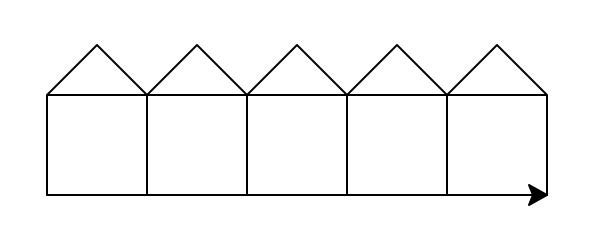
\includegraphics[width=0.3\linewidth]{Grundlagen_Info/00_Programmieren/Skript/Figures/haeuserreihe}
	\end{figure}

\end{myexercise}


% TODO weitere Übungen
\section{Parameter}

Stellen Sie sich vor, sie wollen drei unterschiedlich grosse Quadrate zeichnen. Sie könnten folgendermassen vorgehen:

\lstinputlisting[language=Python,caption=\texttt{noparams.py},label=listing:squares-noparams]{Grundlagen_Info/00_Programmieren/Skript/Code/K04_Functions/squares_noparams.py}

Das ging gerade noch! Was jedoch, wenn Sie 20 unterschiedlich grosse Quadrate zeichnen wollen? Brauchen Sie dann 20 Definitionen? Zum Glück nicht, wie Beispiel \cref{ex:params} zeigt.

\begin{myexample}\label{ex:params}
Folgendes Beispiel verwendet einen \textit{Parameter} \texttt{laenge}, um die Länge des Quadrats jedes Mal anzupassen:
\begin{figure}[H] % not really a figure, just acts as non-floating container
	\begin{lstlisting}[escapechar=!, numbers=left]
import turtle as t

def quadrat(!\colorbox{DeepPink}{la\tikzmark{arrowTo1}enge}!):
	for _ in range(4):
		t.fd(!\colorbox{DeepPink}{la\tikzmark{arrowTo2}enge}!) 
		t.rt(90)

quadrat(!\colorbox{DeepPink}{5\tikzmark{arrow1From}0}!)
quadrat(!\colorbox{DeepPink}{1\tikzmark{arrow2From}00}!)
quadrat(!\colorbox{DeepPink}{1\tikzmark{arrow3From}50}!)
\end{lstlisting}
	\begin{tikzpicture}[overlay,remember picture]
		\draw[red,-stealth] (arrow1From.north) to[bend right] node[right, yshift=-.8cm, fill=RoyalBlue,text=white,rounded corners] {\emoji{handshake} Übergabe} (arrowTo1);
		\draw[red,-stealth] (arrowTo1.south) to[bend right] (arrowTo2);
		\draw[red,-stealth] (arrow2From.south) to[bend right] (arrowTo1);
		\draw[red,-stealth] (arrow3From.south) to[bend right] (arrowTo1);
	\end{tikzpicture}
\end{figure}
\end{myexample}

\subsection{Mehrere Parameter}
Man kann beliebig viele Parameter verwenden in Funktionen. Wichtig dabei ist, diese je durch ein Komma zu trennen.

\begin{myexample}\label{ex:multiple-params}
In folgendem Beispiel kann nicht nur die Anzahl Ecken, sondern auch die Farbe eines Vielecks übergeben werden.
\lstinputlisting[language=Python,caption=\texttt{farb\_vieleck.py},label=listing:farbvieleck]{Grundlagen_Info/00_Programmieren/Skript/Code/K04_Functions/farb_vieleck.py}
\begin{figure}[H]
	\centering
	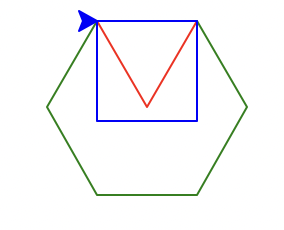
\includegraphics[width=0.2\linewidth]{Grundlagen_Info/00_Programmieren/Figures/mehrere-parameter}
\end{figure}
\end{myexample}

\begin{myexercise}
	Ändern Sie den Code aus \cref{ex:multiple-params} so ab, dass zusätzlich zur Farbe und der Anzahl Ecken auch noch die \textbf{Stiftdicke} für jedes Vieleck verändert werden kann. Verwenden Sie dazu einen weiteren Parameter sowie den Befehl \texttt{t.width(...)}.
\end{myexercise}

\begin{myexercise}
	Erstellen Sie die folgenden Funktionen:
	\begin{itemize}
		\item \lstinline|def summiere(x1, x2)|: Berechnet die Summe zweier Parameter \lstinline|x1| und \lstinline|x2| und gibt das Resultat auf der Konsole aus (mit \lstinline|print|).
		\item \lstinline|def summe_quadrate(x, y)|: Berechnet die Summe \texttt{x}$^2$ + \texttt{y}$^2$ und gibt diese Summe mit \lstinline{print} auf der Konsole aus.
	\end{itemize}
	% TODO implement on Moodle
\end{myexercise}

\subsection{Lebensdauer (\textit{scope}) einer Variable}
Im Code aus \cref{ex:params} wird bei \textit{jedem Aufruf} der Definition \lstinline|quadrat| eine neue Variable \texttt{laenge} erstellt, welche nur \textit{innerhalb} der Funktion existiert und welche jedes Mal einen anderen Wert hat. Den Wert erhält die Variable zum Zeitpunkt des \textit{Aufrufs} der Funktion, also auf den Zeilen 8, 9 und 10!

Die Variable \texttt{laenge} existiert also nur innerhalb der Definition \lstinline|quadrat|. Wenn wir nach Zeile 6 im Hauptprogramm (nicht eingerückt) den Befehl \texttt{print(laenge)} eingeben würden, würden wir eine Fehlermeldung erhalten, da es die Variable nicht mehr gibt. Parameter sind also immer \textbf{\textit{lokale} Variablen}, ebenso wie Variablen, welche wir innerhalb von Funktion erstellen. Diese Variablen \enquote{sterben} nach Ausführung der Definition, daher spricht man auch von der Lebensdauer einer Variable, bzw. von deren Reichweite (en. \textit{scope})

Variablen, welche im Hauptprogramm (nicht eingerückt) erstellt werden, sind sogenannte \textbf{\textit{globale} Variablen}.

\begin{myexercise}\label{ex:local-global}
	Beschreiben Sie, welche der Variablen im unten stehenden Code lokal oder global sind, und welche Variablen auch Parameter sind. Sie sollten insgesamt 5 Variablen finden!
	\lstinputlisting[language=Python,caption=\texttt{houses.py},label=listing:houses]{Grundlagen_Info/00_Programmieren/Skript/Code/K04_Functions/houses.py}

	\begin{myanswer}
		\begin{enumerate}
			\item \lstinline|laenge|: lokale Variable, Parameter der Funktion \lstinline|haus()|
			\item \lstinline|anzahl_mauern|: lokale Variable
			\item \lstinline|laenge_pro_haus|: lokale Variable, Parameter der Funktion \lstinline|haeuserreihe()|
			\item \lstinline|anzahl_haeuser|: lokale Variable
			\item \lstinline|seitenlaenge|: globale Variable
		\end{enumerate}
	\end{myanswer}
\end{myexercise}

\begin{myexercise}
	Was könnte der Vorteil von \textit{lokalen Variablen} sein?
	\begin{myanswer}
		Falls Sie mehrere Funktionen schreiben, können Sie dieselben Variabelnamen und Parameter-Namen innerhalb der Funktionen verwenden, da diese nichts miteinander zu tun haben. Im Code aus \cref{ex:local-global} hätten wir auch in beiden Funktionen \texttt{laenge} schreiben können.
	\end{myanswer}
\end{myexercise}


\section{Werte zurückgeben mit \texorpdfstring{\lstinline|return|}{return}}
\subsection{Einzelne Funktionen}
Wie Sie bereits wissen, können Definitionen mit Kochrezepten verglichen werden: Sie beschreiben einen Ablauf, ohne diesen auszuführen. Damit der Code einer Funktion (\lstinline|def|) ausgeführt wird, müssen Sie die Definition \textbf{aufrufen}: In \cref{ex:multiple-params} wurde dies Beispielsweise mit \lstinline|farb_vieleck(3, "red")| gemacht. Erst aufgrund dieser Zeile wurde etwas gezeichnet!

Dies kann nützlich sein, wenn sie eine Aufgabe mehrmals und in unterschiedlichen Varianten ausführen wollen, wie beispielsweise in \cref{ex:multiple-params}.

Eine wichtige Limitation von Definitionen war bisher, dass Sie zwar Dinge berechnen und auf der Konsole drucken konnten, allerdings verschwinden alle Parameter und lokalen Variablen nach der Ausführung einer Funktion.  Dies bedeutet, dass alle Variablen, die wir je in einer Definition erstellt haben, nur in dieser Definition ``lebten''. Wir konnten jedoch nicht mehr auf Parameter oder lokale Variablen zugreifen, nachdem das Programm beendet wurde.

\begin{myexample}\label{ex:sum-noreturn}
Betrachten Sie folgenden Code. Weshalb führt er zu einer Fehlermeldung?
\begin{lstlisting}[numbers=left]
def summiere(x1, x2):
    summe = x1 + x2
    
summiere(3, 5)
print(summe)
\end{lstlisting}
Die Konsole gibt folgende Meldung aus: \texttt{[Zeile: 5] NameError: name 'summe' is not defined}. Dies bedeutet, dass die Variable \lstinline|summe| auf Zeile 5 nicht existiert. Die Fehlermeldung erklärt sich dadurch, dass alle Variablen, die innerhalb einer Definition erstellt werden, nur innerhalb dieser Definition \enquote{\textit{leben}}, also existieren. Dass Variablen mittels dem Befehl \lstinline|return| auch an das Hauptprogramm ``zurückgegeben'' werden können, lernen wir in diesem Kapitel.
\end{myexample}


Funktionen können jedoch auch Werte an das Hauptprogramm zurückgeben: In diesem Kapitel lernen wir, wie Funktionen, ähnlich wie ``Sous-Chefs'' (Hilfs-Köche) in einer komplexen Küche Zutaten (Parameter) entgegennehmen und Resultate an andere ``Sous-Chefs'' (Funktionen) via das Hauptprogramm weitergeben werden können.

Eine Funktion kann man sich vorstellen wie ein Kochrezept, das einige Zutaten entgegennimmt und ein Resultat (Gericht) zurückgibt. Die Zutaten, oder \enquote{Inputs}, werden dabei häufig als \enquote{\textbf{Parameter}} bezeichnet, währenddem das fertige Gericht, oder \enquote{Resultat} häufig als \enquote{\textbf{\lstinline|return|-Wert}} bezeichnet wird. Diese Idee ist in \cref{fig:funktion-einzeln}) veranschaulicht.

\begin{figure}[H]
	\centering
	\begin{tikzpicture}
		\drawCube{1}{0}{2}{3}
		\node[fill=blue!50, rounded corners] (input1) at (llD11val){3};
		\node[fill=blue!50, rounded corners] (input2) at (llD21val){12};
		\draw[thick,->] (input1) -- (in11);
		\draw[thick,->] (input2) -- (in12);
		\node[fill=green!50, rounded corners](outVal1) at (5,-.6,3){36};
		\draw[thick,->] (out1) -- (outVal1);
	\end{tikzpicture}
	\caption{Illustration einer Funktion mit Inputs (Parametern) und Outputs (\lstinline|return|-Wert)}
	\label{fig:funktion-einzeln}
\end{figure}

\begin{myexample}
Betrachten Sie nochmals den folgenden, leicht modifizierten Code aus \cref{ex:sum-noreturn}. Wenn wir den Wert mit \lstinline|return| an das Hauptprogramm zurückgeben und in einer Variable (im Hauptprogramm, auf Zeile 5) abspeichern, funktioniert der Code nun: Wir können auch ausserhalb der Funktion \lstinline|summiere()| auf einen Wert zugreifen, welcher innerhalb der Definition berechnet wurde, und diesen potentiell weiterverwenden.

\begin{minipage}{\linewidth}
	\begin{figure}[H] % not really a figure, just acts as non-floating container
		\begin{lstlisting}[numbers=left]
def summiere(x1, x2):
    summe = x1 + x2
    return (*@\colorbox{RoyalBlue!50}{sum\tikzmark{arrowFromEx01}me}@*)
    


(*@\colorbox{ForestGreen!50}{re\tikzmark{arrowToEx02}s}@*)=(*@\colorbox{RoyalBlue!50}{summie\tikzmark{arrowToEx01}re(3, 5)}@*)
print(res)
\end{lstlisting}
		\begin{tikzpicture}[overlay,remember picture]
			% Wert zurückgeben
			\draw[RoyalBlue,-stealth, thick] (arrowFromEx01.south) to[bend left] node[align=left, pos=.15, right, fill=RoyalBlue,fill opacity=.5, text opacity=1, text=black,rounded corners] {Wert an das Hauptprogramm zurückgeben...} (arrowToEx01.north);

			\draw[ForestGreen,-stealth, thick] (arrowToEx01.north) to[bend right] node[align=left, pos=.7, above right, fill=ForestGreen,fill opacity=.5, text opacity=1, text=black,rounded corners] {...\textit{und} Wert in Variable speichern, z.B. \lstinline|res|} (arrowToEx02.north);
		\end{tikzpicture}
	\end{figure}
\end{minipage}

\begin{myattention}
	Man muss sich diesen Code wie folgt vorstellen: Auf Zeile 7 wird die Funktion \lstinline|summiere| aufgerufen, die Werte 3 und 5 werden für die Parameter \lstinline|x1| und \lstinline|x2| übergeben. Zeile 2 berechnet nun die Summe dieser beiden Werte. Auf Zeile 3 wird \textcolor{red}{nicht} die Variable \lstinline|summe| an das Hauptprogramm zurückgegeben, sondern deren Wert (in diesem Fall: 8). Dies ist sehr wichtig: Nur weil wir \lstinline|return summe| schreiben, heisst dass nicht, dass wir ausserhalb der Funktion \lstinline|summiere| auf eine Variable \lstinline|summe| zugreifen können. Vielmehr kann man sich vorstellen, dass der blau markierte Bereich auf Zeile 7 nun \enquote{ersetzt} wird durch den Wert 8, welcher vom Unterprogramm an das Hauptprogramm zurückgegeben wird. Zeile 7 liest sich also nach der Ausführung des Unterprogramms so als ob man \lstinline|res = 8| geschrieben hätte. Man könnte selbstverständlich auch einen anderen Variablenname statt \lstinline|res| auswählen, z.B. \lstinline|x|, \lstinline|y|, \lstinline|resultat| (kurz  \lstinline|res|) oder einfach \lstinline|summe|. In letzterem Falle wäre \lstinline|summe| auf Zeile 7 eine globale Variable und somit gänzlich unterschiedlich von der lokalen Variable \lstinline|summe| auf Zeile 2.
\end{myattention}
\end{myexample}

\begin{myexercise}\label{ex:dreieck-return}
	Gegeben seien die Höhe \texttt{h} und die Grundseite \texttt{b} eines Dreiecks. Schreiben Sie eine Funktion \lstinline|def flaeche_dreieck(h, b)|, welche den Flächeninhalt dieses Dreiecks berechnet und mit \lstinline|return| zurückgibt.

	Überprüfen Sie die Korrektheit Ihrer Funktion, indem Sie sie auf Moodle hochladen.
	\begin{myanswer}
		\begin{lstlisting}
def flaeche_dreieck(h, b):
    return h*b/2
\end{lstlisting}
	\end{myanswer}
\end{myexercise}

\begin{myexercise}\label{ex:quadrat-return}
	Geben sei eine ganze Zahl \texttt{n}. Schreiben Sie eine Funktion \lstinline|def square(n)|, welche das Quadrat von \lstinline|n| berechnet und mit \lstinline|return| zurückgibt.

	Überprüfen Sie die Korrektheit Ihrer Funktion, indem Sie sie auf Moodle hochladen.
	\begin{myanswer}
		\begin{lstlisting}
def square(n):
    return n*n
\end{lstlisting}
	\end{myanswer}
\end{myexercise}

\begin{myexercise}\label{ex:print-vs-return}
	In welchen Fällen ist es sinnvoller, einen Wert einfach per \lstinline|print| auf der Konsole auszugeben, und wann ist ein \lstinline|return|-Befehl sinnvoller? Ist das Zurückgeben des Werts in \cref{ex:quadrat-return} und \cref{ex:dreieck-return} sinnvoll, oder würde hier auch ein \lstinline|print| reichen?
	\begin{myanswer}
		\lstinline|return|-Ausdrücke ergeben vor allem dann sinn, wenn mit einem Wert, welcher in einer Funktion berechnet wurde, \textit{ausserhalb der Funktion weitergerechnet} werden soll. In allen anderen Fällen reicht ein \lstinline|print| meist aus. Auch bei \cref{ex:quadrat-return} und \cref{ex:dreieck-return} würde ein einfaches \lstinline|print| reichen.
	\end{myanswer}
\end{myexercise}



\subsection{Mehrere Funktionen}
Wie Sie in \cref{ex:print-vs-return} gesehen haben, ist ein \lstinline|return| in vielen Fällen nicht notwendig, ein einfaches \lstinline|print| reicht in vielen Fällen aus. Wozu kann ein \lstinline|return| eigentlich nützlich sein? Wenn Sie Code schreiben, wird dieser oftmals schnell komplizierter. Somit kann es hilfreich sein, die einzelnen Schritte in Unter-Programme aufzuteilen. Dies erleichtert zudem die \textbf{Modularisierung} und \textbf{Wiederverwendbarkeit} von Code: Beispielsweise könnte eine Funktion, die das Maximum einer Liste berechnet, an verschiedenen Orten in einem längeren Programm mehrmals zum Einsatz kommen

Zum Vergleich: stellen Sie sich vor, Sie arbeiten in einer edlen Michelin-Sterne-Küche an einem raffinierten Gericht, in das viele Arbeitsschritte involviert sind. Häufig müssen in solchen Restaurants bis zu 200 Schritte pro Gericht ausgeführt werden. Daher könnte es sinnvoll sein, einzelne Aufgaben, wie beispielsweise die Herstellung der Saucen, an Ihre Sous-Chefs zu delegieren, und eine Person zu bestimmen, die das ganze Gericht zusammenfügt. Häufig werden Funktionen genau mit solchen komplexen Aufgaben im Hinterkopf geschrieben. Diese Idee ist in \cref{fig:funktionen-mehrere} illustriert.

\begin{figure}[H]
	% Use the \drawCube macro to draw various cubes
	\centering
	\begin{tikzpicture}
		\drawCube{1}{0}{2}{3}
		% feed input values into a1
		\node[fill=blue!50, rounded corners] (input1) at (llD11val){3};
		\node[fill=blue!50, rounded corners] (input2) at (llD21val){12};
		\draw[thick,->] (input1) -- (in11);
		\draw[thick,->] (input2) -- (in12);
		\node[fill=green!50, rounded corners](outVal1) at (5,-.6,3){36};
		\draw[thick,->] (out1) -- (outVal1);
		\drawCube{2}{5.25}{3}{3}
		\drawCube{3}{10.5}{2}{3}
		\draw[thick,->,rounded corners] (out1) -- ++(0,-3.25,0) -- ++(3.15,0,0)node[below]{\lstinline{return out1}} -- ++(4.65,0,0) -- (in31);
	\end{tikzpicture}
	\caption{Illustration einer Code-Struktur, bei welcher mehrere Funktionen zusammenarbeiten}
	\label{fig:funktionen-mehrere}
\end{figure}

In \cref{fig:funktionen-mehrere} haben wir eine Funktion \lstinline|a1|, die zwei Parameter entgegennimmt (\lstinline|x1| und \lstinline|x2|). Mit diesen Parametern macht sie etwas (z.B. die Summe berechnen, ein Quadrat zeichnen oder irgend eine sonstige Aufgabe) und gibt danach einen neuen, berechneten Wert \lstinline|a1| zurück. Dieser kann im Hauptprogramm abgespeichert und an andere Funktionen weitergegeben werden, beispielsweise an die Funktion \lstinline|a3|.

\begin{myexample}
Stellen Sie sich vor, Sie arbeiten für einen Supermarkt und sollten den Preis Ihrer Produkte berechnen. Sie kaufen Ihre Artikel bei einem Grossverteiler ein, daher erhalten Sie auf alle Produkte 10 \% Rabatt. Der Grossverteiler befindet sich im Ausland, Sie müssen also noch 7 \% Mehrwertsteuer hinzufügen. Der Grossverteiler gibt Ihnen den Original-Preis Ihrer Waren \textit{vor} Rabatt und \textit{vor} Mehrwertsteuer.

Folgender Code berechnet den Endpreis, für den Sie ihre Waren verkaufen werden, indem folgende zwei Funktionen aufgerufen werden:
\begin{enumerate}
	\item \lstinline|berechne_rabatt| berechnet den Preis nach Abzug eines Rabatts für ein Produkt.
	\item \lstinline|berechnet_gesamtpreis| ruft \lstinline|berechne_rabatt| auf und fügt zum rabattierten Preis die Mehrwertsteuer hinzu.
\end{enumerate}

\begin{minipage}{\linewidth}
	\begin{figure}[H] % not really a figure, just acts as non-floating container
		\begin{lstlisting}
def berechne_rabatt(preis, rabatt_prozent):
    rabatt = preis * (rabatt_prozent / 100)
    (*@\colorbox{CornflowerBlue}{return preis - \tikzmark{arrowFromEx11} rabatt}@*) # Gibt den Preis nach Abzug des Rabatts zurück


def berechne_gesamtpreis(preis, rabatt_prozent, mwst_prozent):
    (*@\colorbox{CornflowerBlue}{rabatt\tikzmark{arrowToEx11}preis}@*) = berechne_rabatt(preis, rabatt_prozent)
    mwst = rabattpreis * (mwst_prozent / 100)
    return (*@\colorbox{CornflowerBlue}{rabattpre\tikzmark{arrowFromEx12}is + mwst}@*)  # Gibt den Gesamtpreis inklusive Mwst. zurück


# Anwendung
preis = 100  # Basispreis in CHF
rabatt_prozent = 10  # Rabatt in %
mwst_prozent = 7.7  # Mehrwertsteuer in %

(*@\colorbox{CornflowerBlue}{endp\tikzmark{arrowToEx12}reis}@*) = berechne_gesamtpreis(preis, rabatt_prozent, mwst_prozent)
print("Der Endpreis nach Rabatt und Mehrwertsteuer ist:", endpreis)
\end{lstlisting}
		\begin{tikzpicture}[overlay,remember picture]
			% Wert zurückgeben
			\draw[red,-stealth] (arrowFromEx11.north) to[bend left] node[pos=.3, right, fill=RoyalBlue,fill opacity=.5, text opacity=1, text=black,rounded corners] {Wert zurückgeben (und speichern)} (arrowToEx11);
			\draw[red,-stealth] (arrowFromEx12.north) to[bend left] node[pos=.2, right, fill=RoyalBlue, fill opacity=.5, text opacity=1, text=black,rounded corners] {Wert zurückgeben  (und speichern)} (arrowToEx12);
		\end{tikzpicture}
	\end{figure}
\end{minipage}
\end{myexample}


Mit folgendem Code können wir die Turtle eine Spirale aus mehreren Kreisen zeichnen lassen:

\begin{minipage}{.65\textwidth}
	\lstinputlisting[language=Python,caption=\texttt{spirale\_kreis.py}]{Grundlagen_Info/00_Programmieren/Skript/Code/K04_Functions/spirale_kreis.py}
\end{minipage}
\begin{minipage}{.25\textwidth}
	\begin{figure}[H]
		\centering
		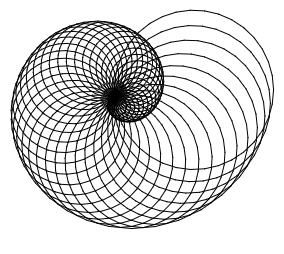
\includegraphics[keepaspectratio, width=\textwidth]{Grundlagen_Info/00_Programmieren/Figures/spirale.png}
	\end{figure}
\end{minipage}

\begin{myexample}
Leider ist unsere Turtle etwas müde und sollte nicht zu viel laufen. Daher möchten wir fortlaufend die Gesamtdistanz berechnen, um am Ende herauszufinden, ob unsere Turtle zu viel Strecke zurückgelegt hat. Dies können wir tun, indem wir die Funktion einen Wert zurückgeben lassen:
\begin{lstlisting}
import turtle as t

def vieleck(umfang, ecken):
    for _ in range(ecken):
        t.fd(umfang/ecken)
        t.rt(360/ecken)

def vieleck_muster(umfang, ecken):
	(*@\colorbox{CornflowerBlue}{gesamtdistanz=0}@*)
    for _ in range(60):
        vieleck(umfang, ecken)
        (*@\colorbox{CornflowerBlue}{gesamtdistanz+=umfang}@*)
        umfang-=10
        t.rt(10)
    (*@\colorbox{CornflowerBlue}{return gesamtdistanz}@*)
    
(*@\colorbox{CornflowerBlue}{gesamtdistanz = }@*)vieleck_muster(600,35)
(*@\colorbox{CornflowerBlue}{print(gesamtdistanz)}@*)
\end{lstlisting}


\end{myexample}


\begin{myexercise}
	Schreiben Sie eine Python-Funktion \lstinline|def notenskala(maxPunkte, erreichtePunkte)|, welche die erreichte Note in Abhängigkeit der maximal möglichen Punktzahl und der erreichten Punktzahl berechnet und per \lstinline|return| zurückgibt. Verwenden Sie dafür die folgende Formel:

	\[ \text{\texttt{note}} = \frac{\text{\texttt{erreichtePunkte}}}{\text{\texttt{maxPunkte}} }\cdot 5 + 1 \]
	\begin{myanswer}
		\begin{lstlisting}
def notenskala(maxPunkte, erreichtePunkte):
    return erreichtePunkte/maxPunkte * 5 + 1
\end{lstlisting}
	\end{myanswer}
\end{myexercise}


\begin{myexercise}[Formel 1 \emoji{chequered-flag}]\label{ex:f1}
	Ein Formel-1-Auto fährt eine bestimmte Strecke in einer bestimmten Zeit. Schreiben Sie eine Funktion \lstinline|def durchschnittsgeschwindigkeit(strecke_km, zeit_min)|, die Strecke in Kilometern und Zeit in Minuten als Eingabe erhält und die durchschnittliche Geschwindigkeit in km/h per \lstinline|return| zurückgibt.

	Formel: Durchschnittsgeschwindigkeit = Strecke (km) / Zeit (h)

	\begin{myanswer}
		\lstinputlisting[language=Python,caption=\texttt{f1\_avg\_speed.py}]{Grundlagen_Info/00_Programmieren/Skript/Code/K04_Functions/f1_avg_speed.py}
	\end{myanswer}
\end{myexercise}

\begin{myexercise}[Boxenstopp \emoji{fuelpump}]
	Ein Formel-1-Rennteam möchte die Gesamtzeit eines Rennens inklusive Boxenstopps berechnen. Gegeben sind die Gesamtstrecke in Km, die Durchschnittsgeschindigkeit in Km/h, die Anzahl Stopps sowie die Dauer pro Stopp in Sekunden.

	Schreiben Sie zwei Funktionen:

	\lstinline|def fahrzeit_ohne_stopps(strecke, kmh)|: Berechnet die reine Fahrzeit in Sekunden und gibt diese per \lstinline|return| zurück.

	\lstinline|def gesamtzeit(strecke, kmh, stopps, stoppdauer)|: Berechnet zuerst die Fahrzeit ohne Stopps (mit der ersten Funktion) und berechnet dann die Gesamtzeit mit Stopps, indem zur Fahrzeit ohne Stopps die Anzahl Boxenstopps mal die Dauer eines Boxenstopps (in Sekunden) hinzugefügt wird. Das Resultat soll ebenfalls per \lstinline|return| zurückgegeben werden.

	Formel 1: Fahrzeit (Sekunden) = Strecke (Km) / Geschindigkeit (Km/h) * 3600

	Formel 2: Gesamtzeit (Sekunden) = Fahrzeit + (Anzahl Stopps $\times$ Stoppdauer)

	\textbf{Tipp 1}: Schreiben Sie den Code zuerst in VSCodium und testen sie ihn erst nachher auf Moodle.

	\textbf{Tipp 2}: Schreiben Sie zuerst die erste Funktion und testen Sie diese mit folgenden Testwerten: Geschwindigkeit = 210 km/h, Strecke = 305 km. Das Resultat sollte sein: 5228.57 Sekunden. Schreiben Sie erst danach die zweite Definition, und rufen Sie darin die erste Definition auf.

	\begin{myanswer}
		\lstinputlisting[language=Python,caption=\texttt{f1\_pitstops.py}]{Grundlagen_Info/00_Programmieren/Skript/Code/K04_Functions/f1_pitstops.py}
	\end{myanswer}
\end{myexercise}

